\begin{figure}[H]
    \centering
    \tikzset{every picture/.style={line width=0.75pt}} %set default line width to 0.75pt        
    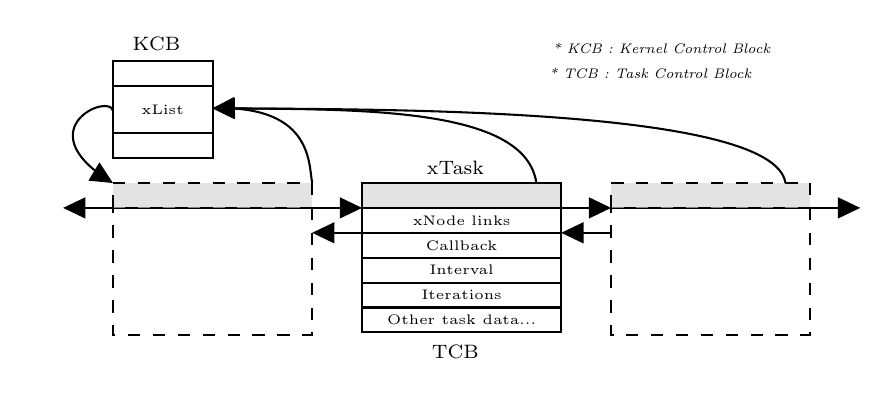
\begin{tikzpicture}[x=0.75pt,y=0.75pt,yscale=-1,xscale=1,scale=1.2]
        \draw   (220,99) -- (300,99) -- (300,109) -- (220,109) -- cycle ;
        \draw  [fill={rgb, 255:red, 210; green, 210; blue, 210 }  ,fill opacity=0.62 ] (220,79) -- (300,79) -- (300,89) -- (220,89) -- cycle ;
        \draw    (220,99) -- (203,99) ;
        \draw [shift={(200,99)}, rotate = 360] [fill={rgb, 255:red, 0; green, 0; blue, 0 }  ][line width=0.08]  [draw opacity=0] (8.93,-4.29) -- (0,0) -- (8.93,4.29) -- cycle    ;
        \draw   (220,109) -- (300,109) -- (300,119) -- (220,119) -- cycle ;
        \draw   (220,119) -- (300,119) -- (300,129) -- (220,129) -- cycle ;
        \draw  [dash pattern={on 4.5pt off 4.5pt}] (320,89) -- (400,89) -- (400,140) -- (320,140) -- cycle ;
        \draw  [fill={rgb, 255:red, 210; green, 210; blue, 210 }  ,fill opacity=0.62 ][dash pattern={on 4.5pt off 4.5pt}] (320,79) -- (400,79) -- (400,89) -- (320,89) -- cycle ;
        \draw   (220,129) -- (300,129) -- (300,139) -- (220,139) -- cycle ;
        \draw  [dash pattern={on 4.5pt off 4.5pt}] (120,89) -- (200,89) -- (200,140) -- (120,140) -- cycle ;
        \draw  [fill={rgb, 255:red, 210; green, 210; blue, 210 }  ,fill opacity=0.62 ][dash pattern={on 4.5pt off 4.5pt}] (120,79) -- (200,79) -- (200,89) -- (120,89) -- cycle ;
        \draw    (200,89) -- (217,89) ;
        \draw [shift={(220,89)}, rotate = 180] [fill={rgb, 255:red, 0; green, 0; blue, 0 }  ][line width=0.08]  [draw opacity=0] (8.93,-4.29) -- (0,0) -- (8.93,4.29) -- cycle    ;
        \draw   (220,89) -- (300,89) -- (300,99) -- (220,99) -- cycle ;
        \draw    (320,99) -- (303,99) ;
        \draw [shift={(300,99)}, rotate = 360] [fill={rgb, 255:red, 0; green, 0; blue, 0 }  ][line width=0.08]  [draw opacity=0] (8.93,-4.29) -- (0,0) -- (8.93,4.29) -- cycle    ;
        \draw    (300,89) -- (317,89) ;
        \draw [shift={(320,89)}, rotate = 180] [fill={rgb, 255:red, 0; green, 0; blue, 0 }  ][line width=0.08]  [draw opacity=0] (8.93,-4.29) -- (0,0) -- (8.93,4.29) -- cycle    ;
        \draw    (120,89) -- (103,89) ;
        \draw [shift={(100,89)}, rotate = 360] [fill={rgb, 255:red, 0; green, 0; blue, 0 }  ][line width=0.08]  [draw opacity=0] (8.93,-4.29) -- (0,0) -- (8.93,4.29) -- cycle    ;
        \draw    (400,89) -- (417,89) ;
        \draw [shift={(420,89)}, rotate = 180] [fill={rgb, 255:red, 0; green, 0; blue, 0 }  ][line width=0.08]  [draw opacity=0] (8.93,-4.29) -- (0,0) -- (8.93,4.29) -- cycle    ;
        \draw   (120,30) -- (160,30) -- (160,40) -- (120,40) -- cycle ;
        \draw   (120,40) -- (160,40) -- (160,59) -- (120,59) -- cycle ;
        \draw   (120,59) -- (160,59) -- (160,69) -- (120,69) -- cycle ;
        \draw    (290,79) .. controls (285.57,48.04) and (217.59,49.52) .. (162.51,49.02) ;
        \draw [shift={(160,49)}, rotate = 360.59000000000003] [fill={rgb, 255:red, 0; green, 0; blue, 0 }  ][line width=0.08]  [draw opacity=0] (8.93,-4.29) -- (0,0) -- (8.93,4.29) -- cycle    ;
        \draw    (200,79) .. controls (198.54,71.76) and (200.4,48.76) .. (162.96,48.94) ;
        \draw [shift={(160,49)}, rotate = 357.98] [fill={rgb, 255:red, 0; green, 0; blue, 0 }  ][line width=0.08]  [draw opacity=0] (8.93,-4.29) -- (0,0) -- (8.93,4.29) -- cycle    ;
        \draw    (390,79) .. controls (385.57,48.04) and (220.56,49.52) .. (162.57,49.02) ;
        \draw [shift={(160,49)}, rotate = 360.59000000000003] [fill={rgb, 255:red, 0; green, 0; blue, 0 }  ][line width=0.08]  [draw opacity=0] (8.93,-4.29) -- (0,0) -- (8.93,4.29) -- cycle    ;
        \draw    (120,50) .. controls (118.54,42.76) and (86.18,56.84) .. (117.47,77.41) ;
        \draw [shift={(120,79)}, rotate = 211.12] [fill={rgb, 255:red, 0; green, 0; blue, 0 }  ][line width=0.08]  [draw opacity=0] (8.93,-4.29) -- (0,0) -- (8.93,4.29) -- cycle    ;
        \draw (260,104) node  [font=\tiny] [align=left] {Callback};
        \draw (260,114) node  [font=\tiny] [align=left] {Interval};
        \draw (260,124) node  [font=\tiny] [align=left] {Iterations};
        \draw (260,134) node  [font=\tiny] [align=left] {Other task data...};
        \draw (257.5,147) node  [font=\scriptsize] [align=left] {TCB};
        \draw (260,94) node  [font=\tiny] [align=left] {xNode links};
        \draw (137.5,23) node  [font=\scriptsize] [align=left] {KCB};
        \draw (140,49.5) node  [font=\tiny] [align=left] {xList};
        \draw (257.5,73) node  [font=\scriptsize] [align=left] {xTask};
        \draw (340.5,25) node  [font=\tiny] [align=left] {\textit{* KCB : Kernel Control Block}};
        \draw (336,35) node  [font=\tiny] [align=left] {\textit{* TCB : Task Control Block}};
    \end{tikzpicture}
\caption{Task node illustration}
\label{fig:tasklist}
\end{figure}